\section{The Solution}
\begin{figure}[htb]
    \begin{center}
        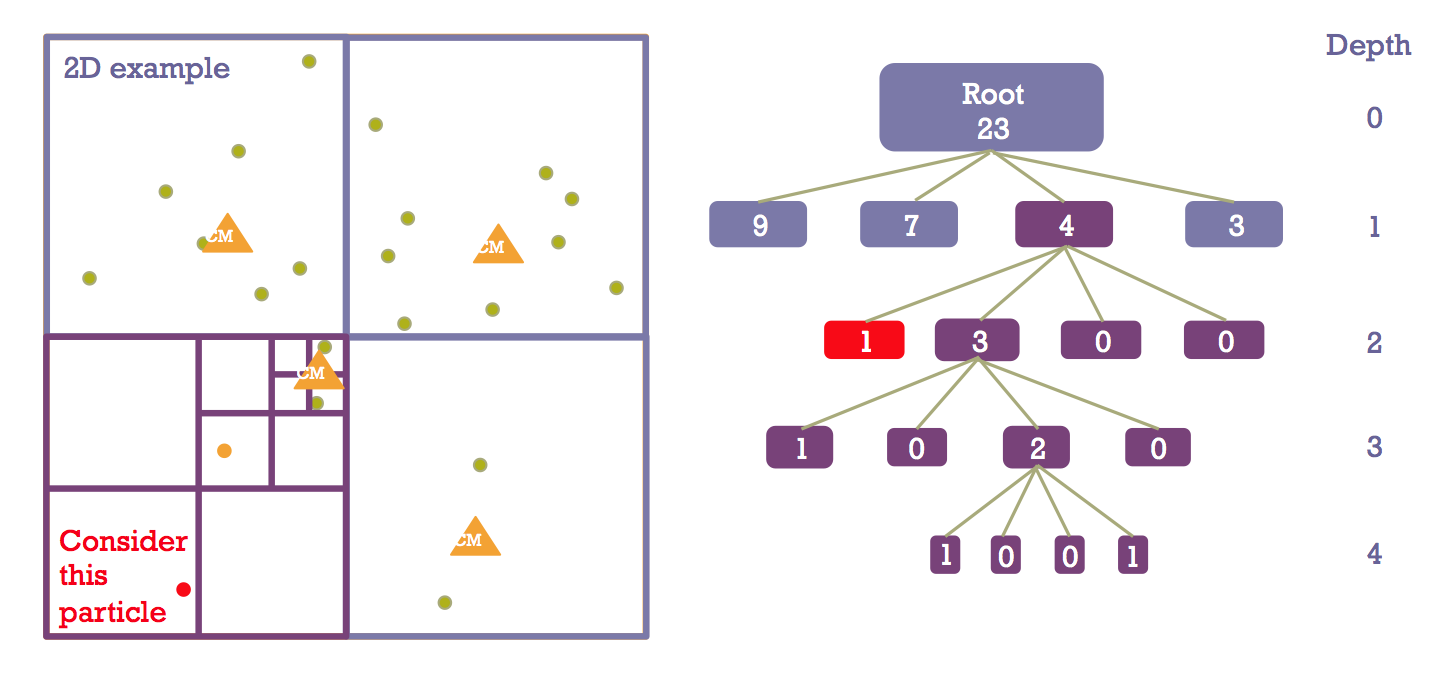
\includegraphics[width=8cm]{../images/tree_walk.png}
        \caption{Diagram of Barnes Hut method}
    \end{center}
\end{figure}
To solve the N body problem, we implemented something known as the Barnes-Hut algorithm. The purpose of this algorithm is to improve computation time, whilst maintaining a high level of accuracy. The idea is to take a group of particles located near to each other and instead of computing forces individually, we do it as group and calculate the force they exert on another particle. To maintain accuracy, we only do this for groups that are far away from the particle. This means that if we have M particles in the group, then we save M-1 force calculations in which we need to compute.

For this assignment, we initially  chose to separate the code into files that represented each section of code we required. We chose to do this for a cleanliness aspect. These files are:
\begin{itemize}
    \item \verb|box_bounds.c| \verb|box_bounds.h|
    \item forces.c forces.h
    \item galsim.c
    \item particle.c particle.h
    \item quad.c quad.h
    \item vector.c vector.h
    \item Makefile
    \item timings.sh
\end{itemize}
\subsection{Quadtree}
To begin with, we constructed the quadtree in the file quad.c. We take an empty tree and insert the particles iteratively, one by one. The first case involves simply adding a particle to an empty tree. The other cases involve recursion.

So in case one, if the tree is empty, we insert the particle into the root node. When we add the particle here, we must also set its mass and centre of mass at the same time, which in this case is easy since it will take the same value as the single particle.
\begin{figure}[htb]
    \begin{center}
        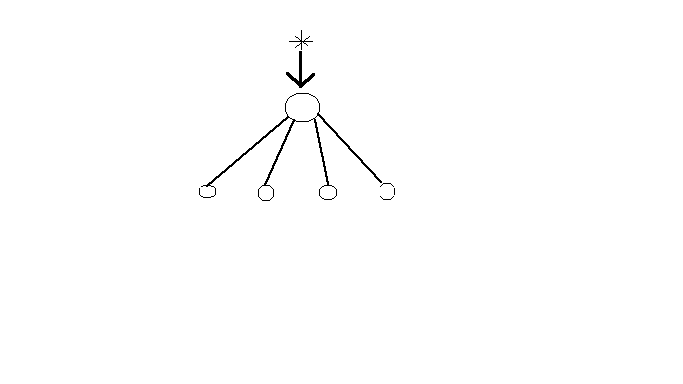
\includegraphics[width=8cm]{../images/empty_tree.png}
        \caption{Diagram of Empty Tree}
    \end{center}
\end{figure}

The second case, is that we traverse the tree and we end up on a node that is taken, but with no children. In this scenario, we must take the particle to one of the children and then also take the particle that was in the node into one of the other children. If they end up going to the same place again, then we traverse the tree until they are split into separate nodes. We update the mass and centre of mass for each particle at the same time.
\begin{figure}[htb]
    \begin{center}
        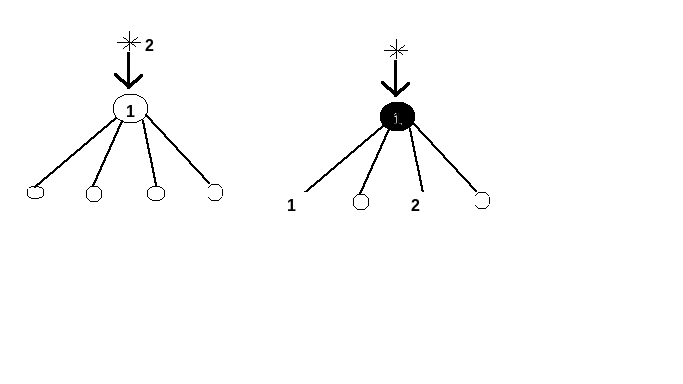
\includegraphics[width=8cm]{../images/node_no_children.png}
        \caption{Diagram of Node with no children}
    \end{center}
\end{figure}
The final case in our code is if we already have a particle in one of the children spots but not all of them. In this scenario, we simply need to traverse the tree until we get to the node with space in its children so that this new particle can be placed here.

The code for this section has been placed in the appendix (A1).
\begin{figure}[htb]
    \begin{center}
        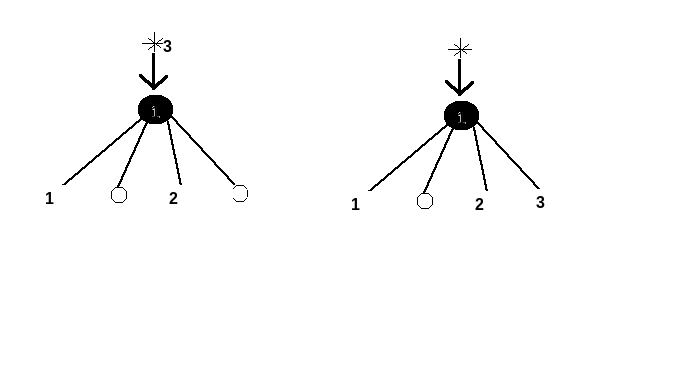
\includegraphics[width=8cm]{../images/children.png}
        \caption{Diagram of Node with children}
    \end{center}
\end{figure}

\newpage
\subsection{Forces}
In order to compute the forces we need the quadtree, which is built in quad.c, the particle that the force is computing for, and \verb|theta_max|. Again, we have three scenarios in which we need to compute the forces. The first case is that if the tree is NULL then we have no forces in which there is any interaction.

The next case we have is if the particle that is inserted next in the tree is firstly not in a particular boxed region and either far enough away from this boxed region or it has no children, then we can compute the force applied to it from the boxed region. We have to check this, since care is needed to not include the particle itself.
The final case we have is to compute the forces of each child and then sum these together to compute the force of the node.

The code for the forces is in the appendix, under section (A2).

\subsection{Other Files}
The purpose of \verb|box_bounds.c| is to house a function called \verb|vector_in_box| which is called into functions in forces. This function is used to determine whether a particle traversing the quad tree is within the bounds of a certain node.

Since our code has been separated out into different files, galsim.c only holds particle position updates and updates outside of the main function. In the main function, we take the arguments from the user, and call the compute force functions to get our output.

The particle.c file contains functions that help read and write the particle data involved.

The vector.c file contains the \verb|r_vector| and norm functions that helps compute the forces on the particles.

For convenience, we have included a timings.sh file that runs the different versions of Makefile on different optimisation flags.
\newpage
